\documentclass[11pt,a4paper]{article}
\usepackage[utf8]{inputenc}
\usepackage{amsmath}
\usepackage{amsfonts}
\usepackage{amssymb}
\usepackage{graphicx}
\usepackage{color}
\usepackage{colortbl}
\usepackage{caption}
\usepackage{wrapfig}
\usepackage{textcomp}
\usepackage[left=2.5cm,right=2.5cm,top=2.5cm,bottom=2.5cm]{geometry}
\usepackage{mathtools, bm}
\usepackage{amssymb, bm}
\usepackage{fancyhdr}
\usepackage{fancybox}
\usepackage{listings}
\usepackage{pgf, tikz}
\pagestyle{fancy}
\fancyhead[L]{Lycée Dumont d'Urville / PB}
\fancyhead[R]{PSI / Informatique / Mesures de rayonnement gamma}
\fancyfoot[C]{page \thepage}

\newcommand{\cadretitre}[2]{\boxput*(0,1){
\colorbox {white}{#1}}{
\setlength{\fboxsep}{6pt}
\fbox {\begin{minipage}{\textwidth -0.7cm}
\bigskip
#2
\bigskip
\end{minipage}}
}}



\title{Mesures de rayonnement gamma}
\date{}
\begin{document}

\maketitle
\thispagestyle{fancy}

Un capteur mesure pendant plusieurs années le rayonnement gamma émis par un lointain pulsar.
Pour chaque gamma reçu, repéré par son rang $i (0 \le i < n)$, on mesure son énergie $a_i$ et l’instant $t_i$ de sa détection.
L’unité d’énergie est le kilo électron-volt (keV), l’unité de temps est le dixième de seconde (1/10 s), l’origine des temps correspond au début de la campagne de mesures.
On supposera $n > 0$.
Pour tout $i$, la quantité $a_i$ est un entier naturel ($a_i \in \mathbb{N}$).
Les valeurs $a_i$ sont rangées dans un tableau $a$ de $n$ éléments de type entier. Ces mesures n’ont pas lieu à intervalles réguliers.
On note les dates $t_i$ (exprimées en 1/10 s, $t_i \in \mathbb{N}$) dans un autre tableau $t$ de $n$ éléments de type entier.
Pour tout $i$ et $j$ tels que $0 \le i < j < n$, on a donc $t_i < t_j$ .

\begin{center}
$a$
\begin{tabular}{|c|c|c|c|c|c|c|c|c|c|c|c|c|c|c|c|c|c|c|c|}
\hline
&&&&&&&&&&&&&&&&&&&\\
\hline
\end{tabular}

$t$
\begin{tabular}{|c|c|c|c|c|c|c|c|c|c|c|c|c|c|c|c|c|c|c|c|}
\hline
&&&&&&&&&&&&&&&&&&&\\
\hline
\end{tabular}
\end{center}

\bigskip

\textbf{Question 1.} Écrire une fonction \texttt{compte(x,a)} qui retourne, en temps linéaire en $n$, le nombre de fois où la valeur $x$ apparaît dans le tableau $a$.

\bigskip

\textbf{Question 2.} En déduire une fonction \texttt{occurrences(a)} qui retourne, en temps quadratique en $n$, un tableau $r$ tel que pour tout $i (0 \le i < n)$, l’élément $r_i$ est le nombre de fois où $a_i$ apparaît dans $a$.

\bigskip

\begin{center}
\huge{partie I}
\end{center}

\bigskip

On cherche à calculer les périodes $T$ de temps pendant lesquelles le rayonnement reste d’énergie constante.

$T = t_j - t_i$ avec $a_i = a_k = a_j$ pour tout $k$ tel que $i \le k \le j$

\bigskip

\textbf{Question 3.} Écrire une fonction \texttt{maxconstant(a,t)} qui retourne, en temps linéaire en $n$, la période la plus grande $T$ pendant laquelle le rayonnement reste constant.

\bigskip

\begin{center}
\huge{partie II}
\end{center}

\bigskip

Soit $occ$ le tableau calculé à la question 2.

\bigskip

\textbf{Question 4.} Écrire une fonction \texttt{maxoccurrences(a,occ)} qui retourne, en temps linéaire en $n$, les indices $i_1$ et $i_2$ de deux rayonnements $m_1$ et $m_2$ qui apparaissent le plus grand nombre de fois dans le tableau de mesures $a$.
(Si le tableau $a$ contient des valeurs toutes identiques, on posera $i_2=m_2 = -1$).

On veut maintenant réorganiser les tableaux de mesures $a$ et de dates $t$ pour mettre en tête toutes les mesures donnant $m_1$, puis celles valant $m_2$, puis toutes les autres.
La réorganisation des tableaux $a$ et $t$ demandée est donc telle que :

$0\le k<b \Rightarrow a_k=m_1$

$b\le k<r \Rightarrow a_k=m_2$

$r\le k<n \Rightarrow a_k \notin {m_1,m_2}$

Après réorganisation, le tableau $t$ vérifie toujours que $t_i$ est la date à laquelle s’est produit le rayonnement $a_i (0 \le i < n)$.

\bigskip

\textbf{Question 5.} Écrire une fonction \texttt{trier(a,t,m1,m2)} qui réordonne, en temps linéaire en $n$, les tableaux $a$ et $t$ pour regrouper en tête les deux mesures les plus fréquentes, comme indiqué précédemment.

Indication : on parcourra les tableaux $a$ et $t$ (dans le sens des indices croissants) en maintenant une décomposition de la forme suivante :

\begin{figure}[h]
\begin{center}
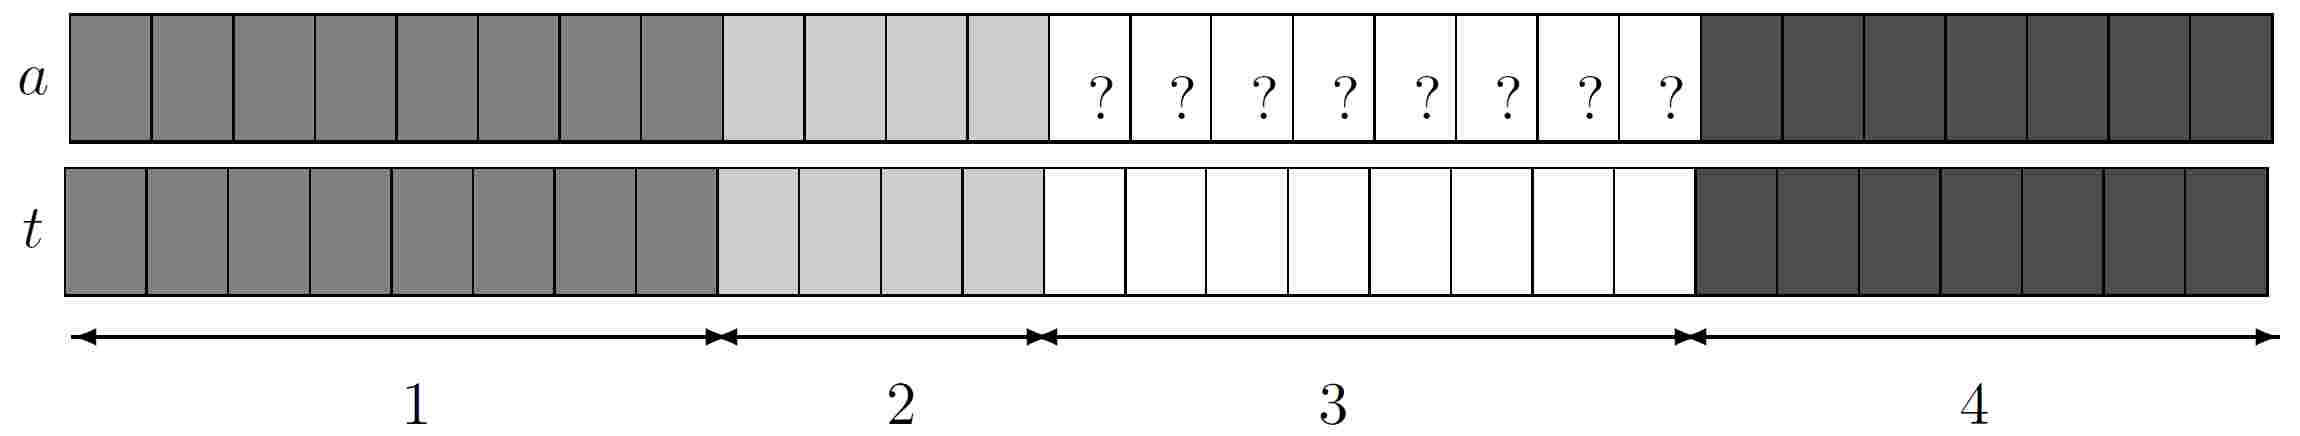
\includegraphics[scale=0.15]{Image1.jpg} 
\end{center}
\end{figure}

avec $a_i$ valant respectivement $m_1$, $m_2$ et une valeur non prise dans {$m_1, m_2$} dans les zones 1, 2 et 4.

Au début les tableaux $a$ et $t$ sont de la forme :

\bigskip


\begin{figure}[h]
\begin{center}
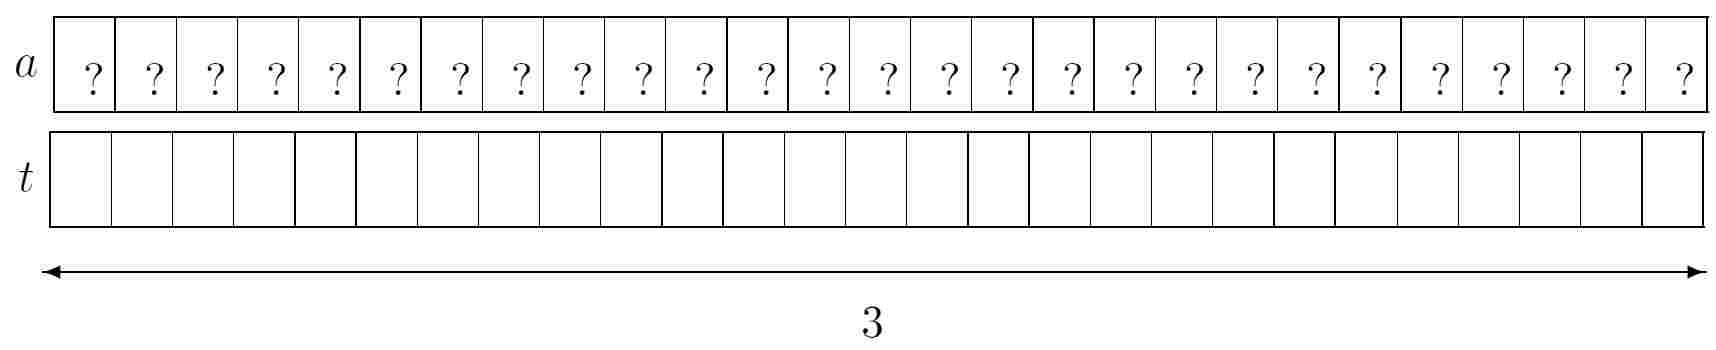
\includegraphics[scale=0.21]{Image2.jpg} 
\end{center}
\end{figure}

À la fin les mêmes tableaux $a$ et $t$ sont de la forme :

\bigskip

\begin{figure}[h]
\begin{center}
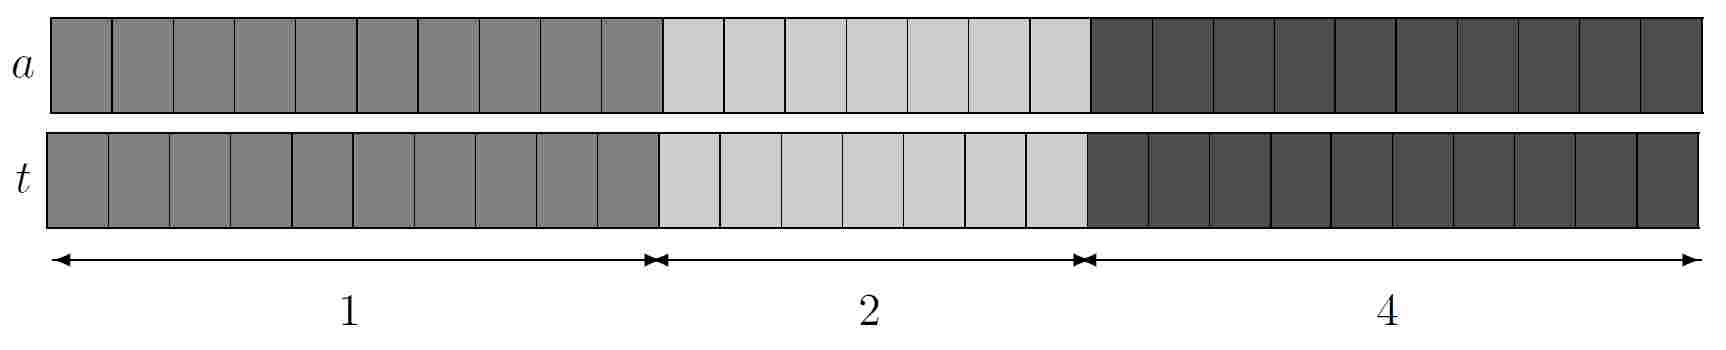
\includegraphics[scale=0.21]{Image3.jpg} 
\end{center}
\end{figure}

\textbf{Question 6.} La fonction précédente garde-t-elle la croissance des dates à l’intérieur de chaque zone, c’est-à-dire que $i < j$ implique $t_i < t_j$ pour $i$ et $j$ dans une même zone ? Justifier votre réponse.

\end{document}

